    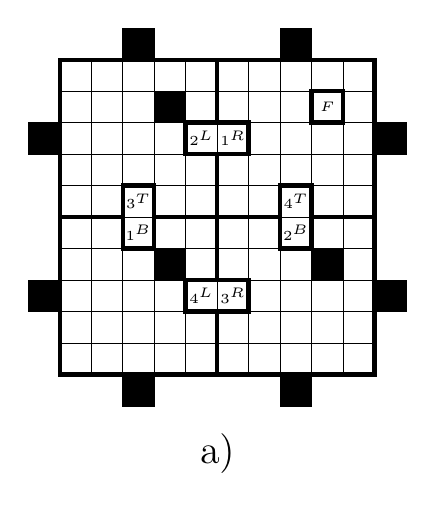
\begin{tikzpicture}
        \draw[step=0.4,thin,shift={(0.2,0.2)}] (0.8,0.8) grid (4.8,4.8);
        \draw[ultra thick] (1,1) rectangle (5,5);
        \draw[ultra thick] (3,1) -- (3,1.8);
        \draw[ultra thick] (3,2.2) -- (3,3.8);
        \draw[ultra thick] (3,4.2) -- (3,5);
        \draw[ultra thick] (1,3) -- (1.8,3);
        \draw[ultra thick] (2.2,3) -- (3.8,3);
        \draw[ultra thick] (4.2,3) -- (5,3);
        
        \draw[fill] (0.6,1.8) rectangle (1,2.2);
        \draw[fill] (0.6,3.8) rectangle (1,4.2);
        \draw[fill] (1.8,5) rectangle (2.2,5.4);
        \draw[fill] (1.8,0.6) rectangle (2.2,1);
        \draw[fill] (3.8,0.6) rectangle (4.2,1);
        \draw[fill] (5,1.8) rectangle (5.4,2.2);
        \draw[fill] (5,3.8) rectangle (5.4,4.2);
        \draw[fill] (3.8,5) rectangle (4.2,5.4);
        
        \draw[fill] (2.2,2.2) rectangle (2.6,2.6);
        \draw[fill] (4.2,2.2) rectangle (4.6,2.6);
        \draw[fill] (2.2,4.2) rectangle (2.6,4.6);
        
        \draw[ultra thick] (4.2,4.2) rectangle (4.6,4.6);
        \draw[ultra thick] (3.8,2.6) rectangle (4.2,3.4);
        \draw[ultra thick] (1.8,2.6) rectangle (2.2,3.4);
        \draw[ultra thick] (2.6,3.8) rectangle (3.4,4.2);
        \draw[ultra thick] (2.6,1.8) rectangle (3.4,2.2);
    
        \node at (4.4,4.4) {\tiny $F$};
        \node at (2,3.2) {\tiny $3^T$};
        \node at (2,2.8) {\tiny $1^B$};
        \node at (4,3.2) {\tiny $4^T$};
        \node at (4,2.8) {\tiny $2^B$};
        \node at (2.8,4) {\tiny $2^L$};
        \node at (2.8,2) {\tiny $4^L$};
        \node at (3.2,4) {\tiny $1^R$};
        \node at (3.2,2) {\tiny $3^R$};

        \node at (3,0){ \Large a)};
    
    \end{tikzpicture}
